% !TEX root = ../pdf/lsj.tex
% [There are multiple lsj.tex files, but the one in ../pdf is the usual one]


%%%%%%%%%%%%%%%%%%%%%%%%%%%%%%%%%%%%%%%%%%%%%%%
\chapter{Drawing graphs\label{ch:graphics}}

\begin{quote}
{\it Above all else show the data.}\\
\hspace*{2cm} --Edward Tufte\FOOTNOTE{The origin of this quote is Tufte's lovely book {\it The Visual Display of Quantitative Information}.}
\end{quote}

\noindent
Visualising data is one of the most important tasks facing the data analyst. It's important for two distinct but closely related reasons. Firstly, there's the matter of drawing ``presentation graphics'': displaying your data in a clean, visually appealing fashion makes it easier for your reader to understand what you're trying to tell them. Equally important, perhaps even more important, is the fact that drawing graphs helps {\it you} to understand the data. To that end, it's important to draw ``exploratory graphics'' that help you learn about the data as you go about analysing it. These points might seem pretty obvious, but I cannot count the number of times I've seen people forget them. 

To give a sense of the importance of this chapter, I want to start with a classic illustration of just how powerful a good graph can be. To that end, Figure~\ref{fig:snowmap1} shows a redrawing of one of the most famous data visualisations of all time: John Snow's 1854 map of cholera deaths. The map is elegant in its simplicity. In the background we have a street map, which helps orient the viewer. Over the top, we see a large number of small dots, each one representing the location of a cholera case. The larger symbols show the location of water pumps, labelled by name. Even the most casual inspection of the graph makes it very clear that the source of the outbreak is almost certainly the Broad Street pump. Upon viewing this graph, Dr Snow arranged to have the handle removed from the pump, ending the outbreak that had killed over 500 people. Such is the power of a good data visualisation.


The goals in this chapter are twofold: firstly, to discuss several fairly standard graphs that we use a lot when analysing and presenting data, and secondly, to show you how to create these graphs in jamovi. The graphs themselves tend to be pretty straightforward, so in that respect this chapter is pretty simple. Where people usually struggle is learning how to produce graphs, and especially, learning how to produce good graphs. Fortunately, learning how to draw graphs in jamovi is reasonably simple, as long as you're not too picky about what your graph looks like. What I mean when I say this is that jamovi has a lot of {\it very} good default graphs, or plots, that most of the time produce a clean, high-quality graphic. However, on those occasions when you do want to do something non-standard, or if you need to make highly specific changes to the figure, then the graphics functionality in jamovi is not yet capable of supporting advanced work or detail editing. 

The structure of this chapter is as follows: I'll start out by giving you a very quick overview of how graphics work in jamovi. I'll then discuss several different kinds of graph and how to draw them. 

\begin{figure}[t!!]
\begin{center}
\epsfig{file = ../img/graphics/snowMap.eps, clip=true,width = 12cm}
\caption{A stylised redrawing of John Snow's original cholera map. Each small dot represents the location of a cholera case, and each large circle shows the location of a well. As the plot makes clear, the cholera outbreak is centred very closely on the Broad St pump.  This image uses the data from the \rtext{HistData} package \protect\cite{Friendly2011}, and was drawn using minor alterations to the commands provided in the help files. Note that Snow's original hand drawn map used different symbols and labels, but you get the idea.}
\label{fig:snowmap1}
\HR
\end{center}
\end{figure}


\section{Histograms\label{sec:hist}}
 
Let's begin with the humble \keyterm{histogram}. Histograms are one of the simplest and most useful ways of visualising data. They make most sense when you have an interval or ratio scale (e.g., the \rtext{afl.margins} data from Chapter~\ref{ch:descriptives}) and what you want to do is get an overall impression of the data. Most of you probably know how histograms work, since they're so widely used, but for the sake of completeness I'll describe them. All you do is divide up the possible values into \keyterm{bins}, and then count the number of observations that fall within each bin. This count is referred to as the frequency or density of the bin, and is displayed as a vertical bar: in the AFL winning margins data, there are 33 games in which the winning margin was less than 10 points, and it is this fact that is represented by the height of the leftmost bar that we showed earlier in \ref{ch:descriptives}, Figure~\ref{fig:histogram1}. With these earlier graphs we have used an advanced plotting package in \R\ which, for now, is beyond the capability of jamovi. But jamovi gets us close, and drawing this histogram in jamovi is pretty straightforward: open up the `plots' options under `Exploration' - `Descriptives' and click the `histogram' check box, as in Figure \ref{fig:jamovi_histogram}. jamovi defaults to labelling the y-axis as `density' and the x-axis with the variable name. The \keyterm{bins} are selected automatically, and there is no scale, or count, information on the y-axis, unlike the previous Figure~\ref{fig:histogram1}. But this does not matter too much, because after all what we are really interested in is our impression of the shape of the distribution - is it normally distributed, or is there a skew or kurtosis? Our first impressions of these characteristics come from drawing a \keyterm{histogram}.

\begin{figure}[h]
\begin{center}
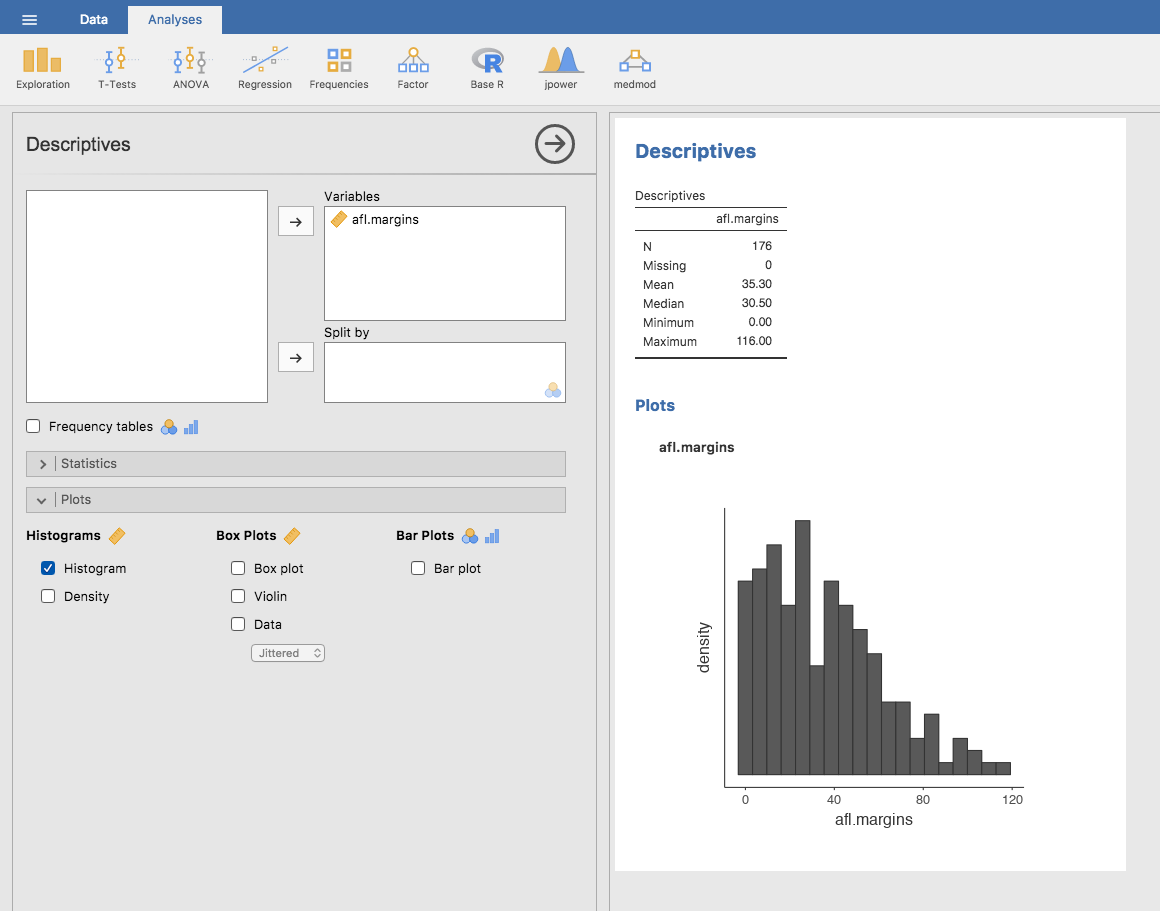
\epsfig{file = ../img/graphics/jamovi_histogram.png, clip=true,width = 12cm}
\caption{jamovi screen showing the histogram check box}
\label{fig:jamovi_histogram}
\HR
\end{center}
\end{figure}

One additional feature that jamovi provides is the ability to plot a `Density' curve. You can do this by clicking the `Density' check box under the `Plots' options (and unchecking `Histogram'), and this gives us the plot shown in Figure \ref{fig:histogram2}. A density plot visualises the distribution of data over a continuous interval or time period. This chart is a variation of a histogram that uses \keyterm{kernel smoothing} to plot values, allowing for smoother distributions by smoothing out the noise. The peaks of a density plot help display where values are concentrated over the interval. An advantage density plots have over histograms is that they're better at determining the distribution shape because they're not affected by the number of bins used (each bar used in a typical histogram). A histogram comprising of only 4 bins wouldn't produce a distinguishable enough shape of distribution as a 20-bin histogram would. However, with density plots, this isn't an issue. 

\begin{figure}[h]
\begin{center}
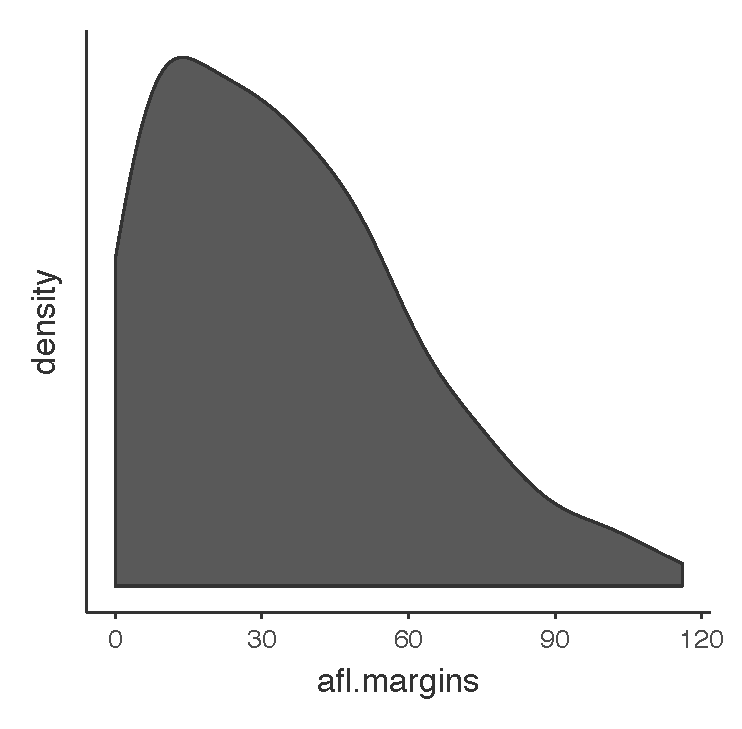
\epsfig{file = ../img/graphics/histogram2.pdf, clip=true,width = 12cm}
\caption{A density plot of the \rtext{afl.margins} variable plotted in jamovi}
\label{fig:histogram2}
\HR
\end{center}
\end{figure}

Although this image would need a lot of cleaning up in order to make a good presentation graphic (i.e., one you'd include in a report), it nevertheless does a pretty good job of describing the data. In fact, the big strength of a histogram or density plot is that (properly used) it does show the entire spread of the data, so you can get a pretty good sense about what it looks like. The downside to histograms is that they aren't very compact: unlike some of the other plots I'll talk about it's hard to cram 20-30 histograms into a single image without overwhelming the viewer. And of course, if your data are nominal scale then histograms are useless.


\section{Boxplots~\label{sec:boxplots}}

Another alternative to histograms is a \keyterm{boxplot}, sometimes called a ``box and whiskers'' plot. Like histograms, they're most suited to interval or ratio scale data. The idea behind a boxplot is to provide a simple visual depiction of the median, the interquartile range, and the range of the data. And because they do so in a fairly compact way, boxplots have become a very popular statistical graphic, especially during the exploratory stage of data analysis when you're trying to understand the data yourself. Let's have a look at how they work, again using the \rtext{afl.margins} data as our example. 

The easiest way to describe what a boxplot looks like is just to draw one. Click on the `Box plot' check box, and you will get the plot shown on the lower right of Figure \ref{fig:boxplot1}. jamovi has drawn the most basic boxplot possible. When you look at this plot, this is how you should interpret it: the thick line in the middle of the box is the median; the box itself spans the range from the 25th percentile to the 75th percentile; and the ``whiskers'' cover the full range from the minimum value to the maximum value. 

\begin{figure}[h]
\begin{center}
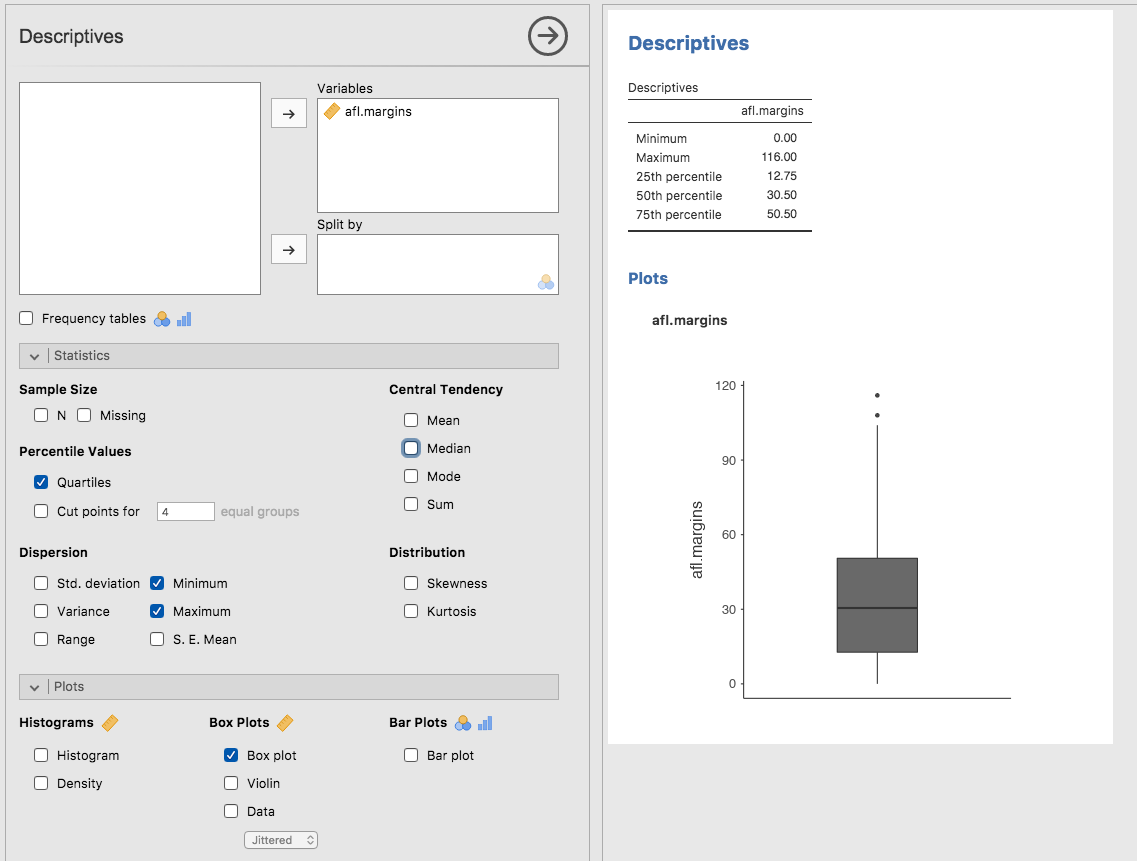
\epsfig{file = ../img/graphics/boxplot1.png, clip=true,width = 12cm}
\caption{A box plot of the \rtext{afl.margins} variable plotted in jamovi}
\label{fig:boxplot1}
\HR
\end{center}
\end{figure}

In practice, this isn't quite how boxplots usually work. In most applications, the ``whiskers'' don't cover the full range from minimum to maximum. Instead, they actually go out to the most extreme data point that doesn't exceed a certain bound. By default, this value is 1.5 times the interquartile range (IQR), calculated as \rtext{25th percentile - (1.5*IQR)} for the lower boundary, and \rtext{75th percentile + (1.5*IQR)} for the upper boundary. Any observation whose value falls outside this range is plotted as a circle or dot instead of being covered by the whiskers, and is commonly referred to as an \keyterm{outlier}. For our AFL margins data, there are two observations that fall outside this range, and these observations are plotted as dots (the upper boundary is 107, and looking over the data column in the spreadsheet there are two observations with values higher than this: 108 and 116 - these are the dots). 


\SUBSECTION{Violin plots~\label{sec:violinplots}}

A variation to the traditional box plot is the violin plot. Violin plots are similar to box plots, except that they also show the kernel probability density of the data at different values. Typically, violin plots will include a marker for the median of the data and a box indicating the interquartile range, as in standard box plots. In jamovi you can achieve this sort of functionality by checking both the `Violin' and the 'Box plot' check boxes. See Figure \ref{fig:boxplot2}, which also has the `Data' check box turned on to show the actual data points on the plot. This does tend to make the graph a bit too busy though, in my opinion. Clarity is simplicity, so in practice it might be better to just use a simple box plot.


\begin{figure}[h]
\begin{center}
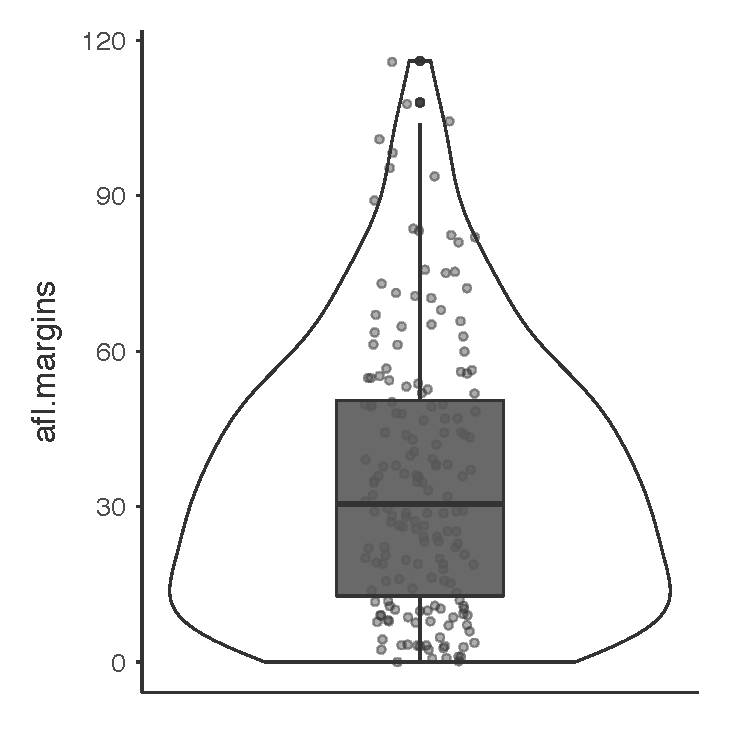
\epsfig{file = ../img/graphics/boxplot2.pdf, clip=true,width = 12cm}
\caption{A violin plot of the \rtext{afl.margins} variable plotted in jamovi, alsow showing a box plot and data points}
\label{fig:boxplot2}
\HR
\end{center}
\end{figure}



\SUBSECTION{Drawing multiple boxplots~\label{sec:multipleboxplots}}

One last thing. What if you want to draw multiple boxplots at once? Suppose, for instance, I wanted separate boxplots showing the AFL margins not just for 2010, but for every year between 1987 and 2010. To do that, the first thing we'll have to do is find the data. These are stored in the \filename{aflsmall2.csv} file. So let's load it into jamovi and see what is in it. You will see that it a pretty big data set. It contains 4296 games, and contains the variables that we're interested in. What we want to do is have jamovi draw boxplots for the \rtext{margin} variable, plotted separately for each separate \rtext{year}. The way to do this is to move the \rtext{year} variable across into the `Split by' box, as in Figure \ref{fig:splitfile1}

\begin{figure}[h]
\begin{center}
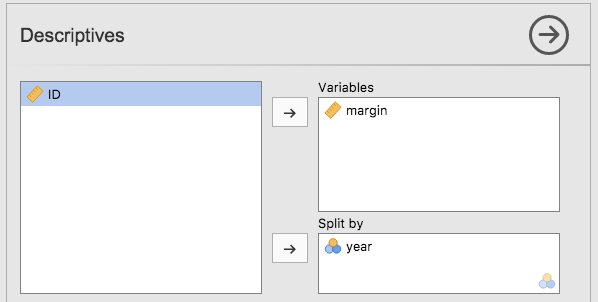
\epsfig{file = ../img/graphics/splitfile1.png, clip=true,width = 12cm}
\caption{jamovi screen shot showing the `Split by' window}
\label{fig:splitfile1}
\HR
\end{center}
\end{figure}

The result is shown in Figure~\ref{fig:boxplot3}. This version of the box plot, split by year, gives a sense of why it's sometimes useful to choose box plots instead of histograms. Even before taking the time to turn this basic output into something more readable, it's possible to get a good sense of what the data look like from year to year without getting overwhelmed with too much detail. Now imagine what would have happened if I'd tried to cram 24 histograms into this space: no chance at all that the reader is going to learn anything useful.

\begin{figure}[h!!]
\begin{center}
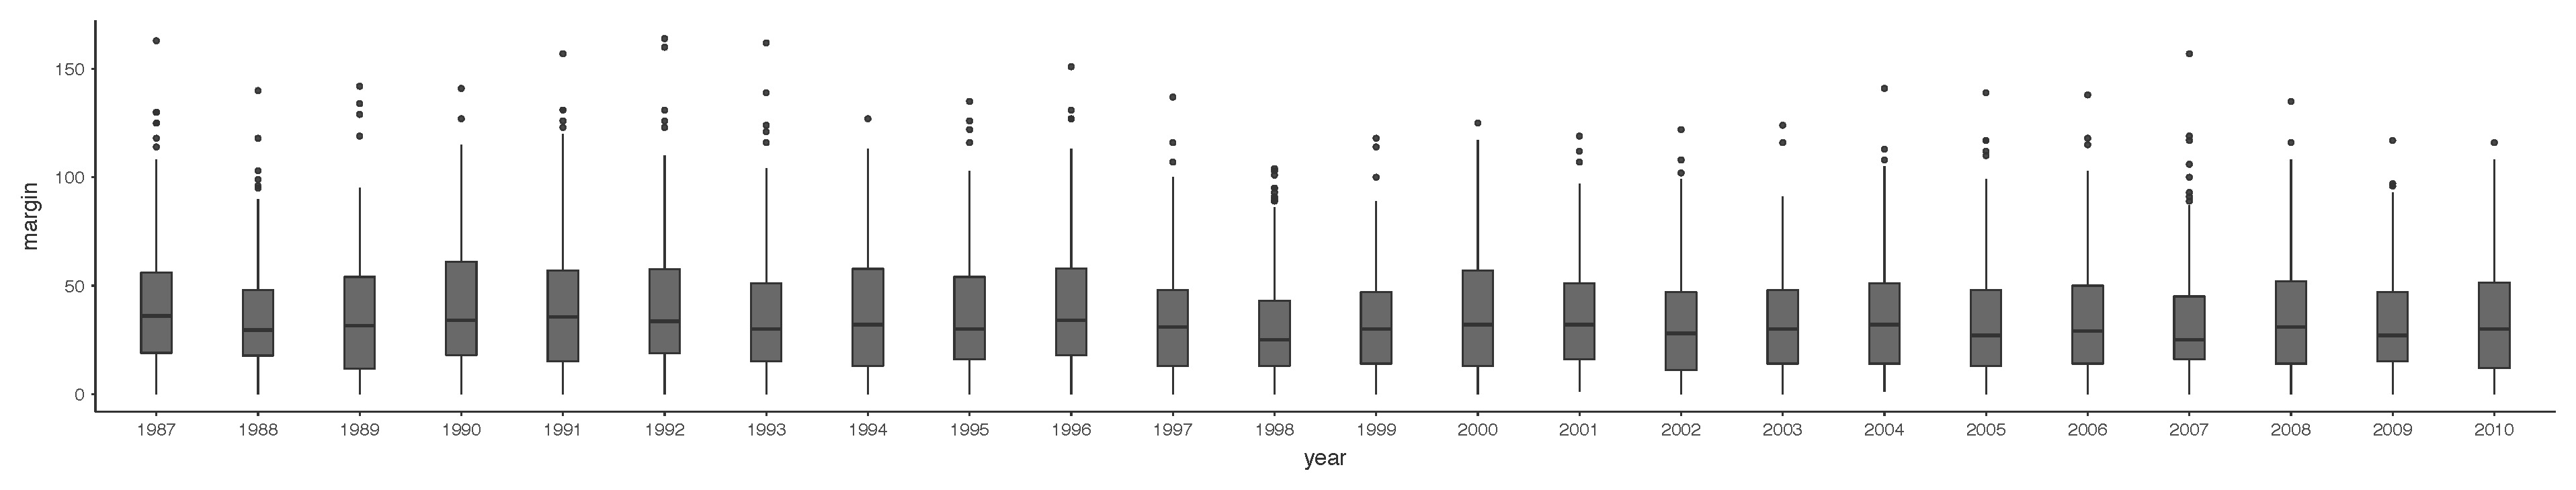
\epsfig{file = ../img/graphics/boxplot3.pdf, clip=true,width = 14cm, height = 5cm}
\caption{Multiple boxplots plotted in jamovi, for the \rtext{margin} by \rtext{year} variables in the \rtext{aflsmall2} data set}
\label{fig:boxplot3}
\HR
\end{center}
\end{figure}


\SUBSECTION{Using box plots to detect outliers~\label{sec:boxplotoutliers}}

\begin{figure}[h]
\begin{center}
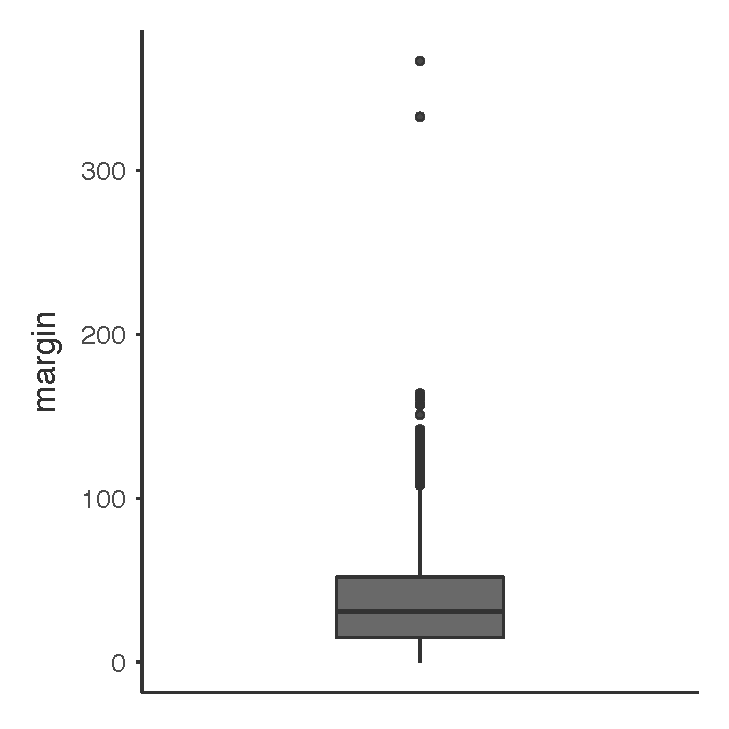
\epsfig{file = ../img/graphics/boxplot4.pdf, clip=true,width =12cm} 
\caption{A boxplot showing two very suspicious outliers!}
\label{fig:boxplot4}
\HR
\end{center}
\end{figure}

Because the boxplot automatically separates out those observations that lie within a certain range, depicting them with a dot in jamovi, people often use them as an informal method for detecting \keyterm{outliers}: observations that are ``suspiciously'' distant from the rest of the data. Here's an example. Suppose that I'd drawn the boxplot for the AFL margins data, and it came up looking like Figure~\ref{fig:boxplot4}. It's pretty clear that something funny is going on with two of the observations. Apparently, there were two games in which the margin was over 300 points! That doesn't sound right to me. Now that I've become suspicious, it's time to look a bit more closely at the data. In jamovi you can quickly find out which of these observations are suspicious, and then you can go back to the raw data to see if there has been a mistake in data entry. To do this you need to set up a filter, so that only those observations with values over a certain threshold are included. In our example, the threshold is over 300, so that is the filter we will create. First, click on the `Filters' button at the top[ of the jamovi window, and then type `margin > 300' into the filter field, as in Figure \ref{fig:filter1}. This filter creates a new column in the spreadsheet view where only those observations that pass the filter are included. One neat way to quickly identify which observations these are is to tell jamovi to produce a `Frequency table' (in the `Exploration' - `Descriptives' window) for the ID variable (which must be a nominal variable, otherwise the Frequency table is not produced). In Figure \ref{fig:filter2} you can see that the ID values for the observations where the margin was over 300 are \rtext{14} and \rtext{134}. These are suspicious cases, or observations, where you should go back to the original data source to find out what is going on.


\begin{figure}[h]
\begin{center}
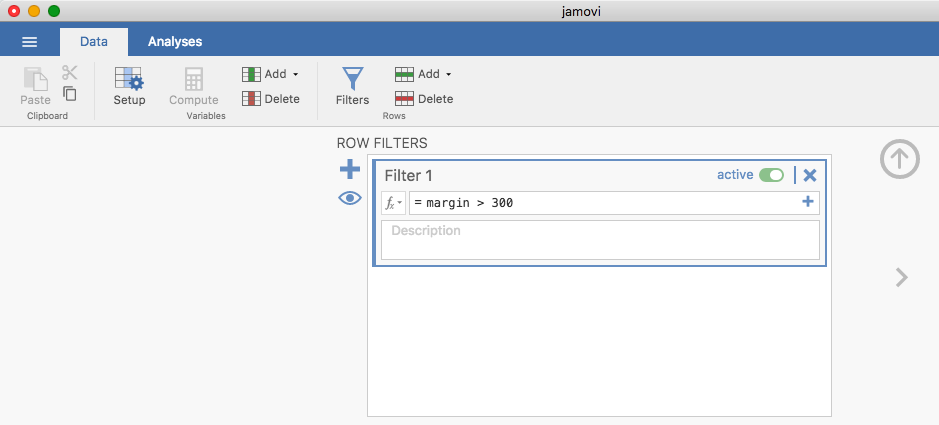
\epsfig{file = ../img/graphics/filter1.png, clip=true,width =12cm} 
\caption{the jamovi filter screen}
\label{fig:filter1}
\HR
\end{center}
\end{figure}

\begin{figure}[h!!]
\begin{center}
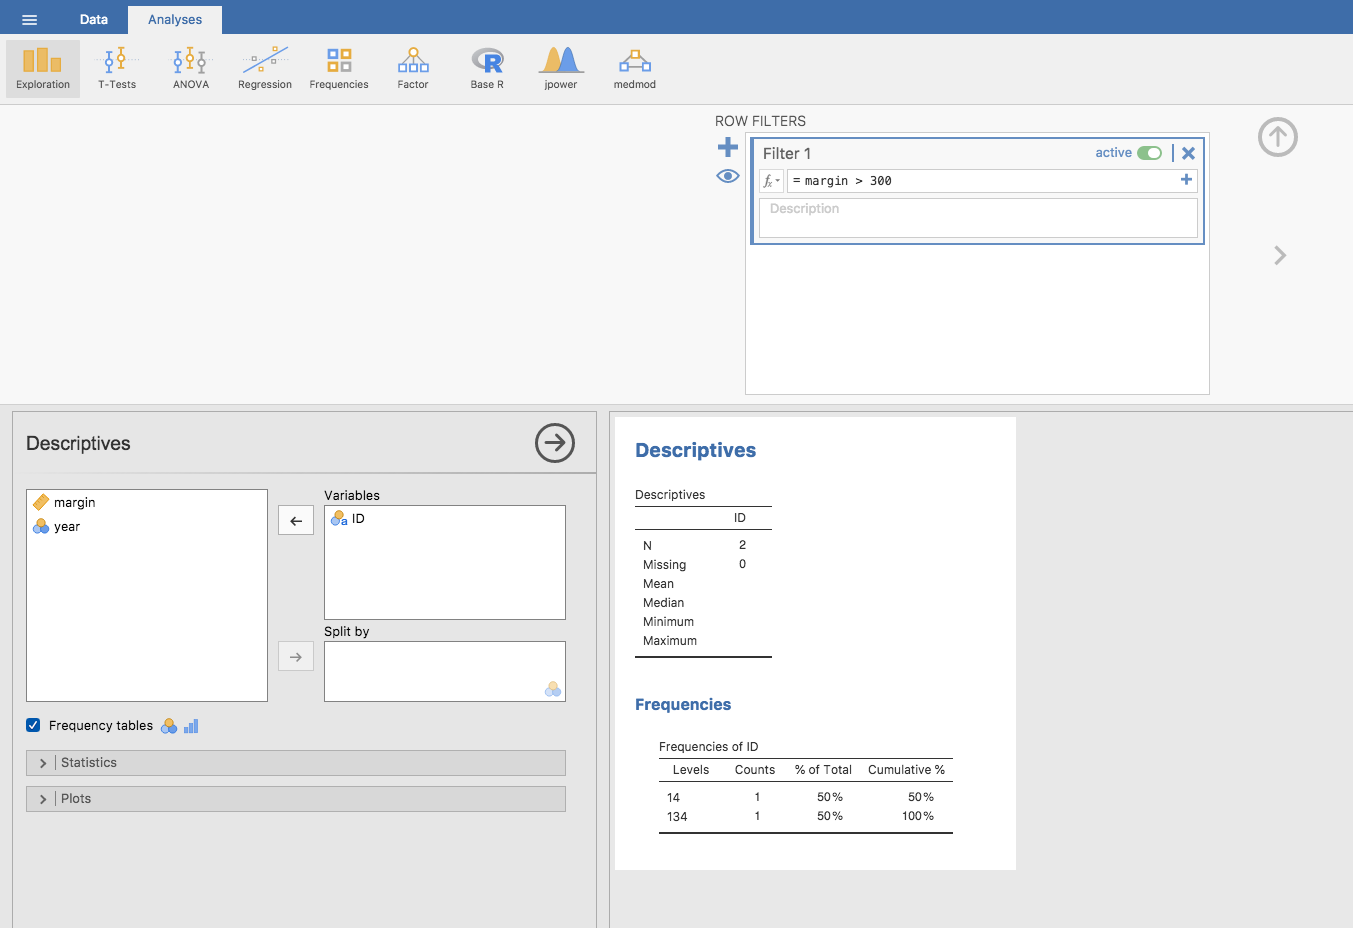
\epsfig{file = ../img/graphics/filter2.png, clip=true,width =12cm} 
\caption{Frequency table for \rtext{ID} showing the ID numbers for the two suspicious outliers: \rtext{14} and \rtext{134}}
\label{fig:filter2}
\HR
\end{center}
\end{figure}


usually you find that someone has just typed in the wrong number. While this might seem like a silly example, I should stress that this kind of thing actually happens a lot. Real world data sets are often riddled with stupid errors, especially when someone had to type something into a computer at some point. In fact, there's actually a name for this phase of data analysis, since in practice it can waste a huge chunk of our time: \keyterm{data cleaning}. It involves searching for typos, missing data and all sorts of other obnoxious errors in raw data files.

For less extreme values, even if they are flagged in a a boxplot as outliers, the decision about whether to include outliers or exclude them in any analysis depends heavily on {\it why} you think the data look they way they do, and what you want to use the data {\it for}. You really need to exercise good judgement here: if the outlier looks legitimate to you, then keep it. In any case, I'll return to the topic again in Section~\ref{sec:regressiondiagnostics}. 



\section{Bar graphs\label{sec:bargraph}}

Another form of graph that you often want to plot is the \keyterm{bar graph}. Let's use the \rtest{afl.finalists} data set with the \rtext{afl.finalists} variable that I introduced in Section~\ref{sec:mode}. What I want to do is draw a bar graph that displays the number of finals that each team has played in over the time spanned by the \rtext{afl} data set. There are lots of teams, but I am particularly interested in just four: Brisbane, Carlton, Fremantle and Richmond. So the first step is to set up a filter so just those four teams are included in the bar graph. This is straightforward in jamovi, and you can do it by using the `Filters' function that we used previously. Open up the `Filters' screen and type in the following: \\

\rtext{afl.finalists == 'Brisbane' or afl.finalists == 'Carlton' or afl.finalists == 'Fremantle' or afl.finalists == 'Richmond'} \\

When you have done this you will see, in the `Data' view, that jamovi has filtered out all values apart from those we have specified. Next, open up the `Exploration' - `Descriptives' window and click on the `Bar plot' check box (remember to move the `afl.finalists' variable across into the `Variables' box so that jamovi knows which variable to use). You should then get a bar graph, something like that shown in Figure~\ref{fig:bar1}.

\begin{figure}[h]
\begin{center}
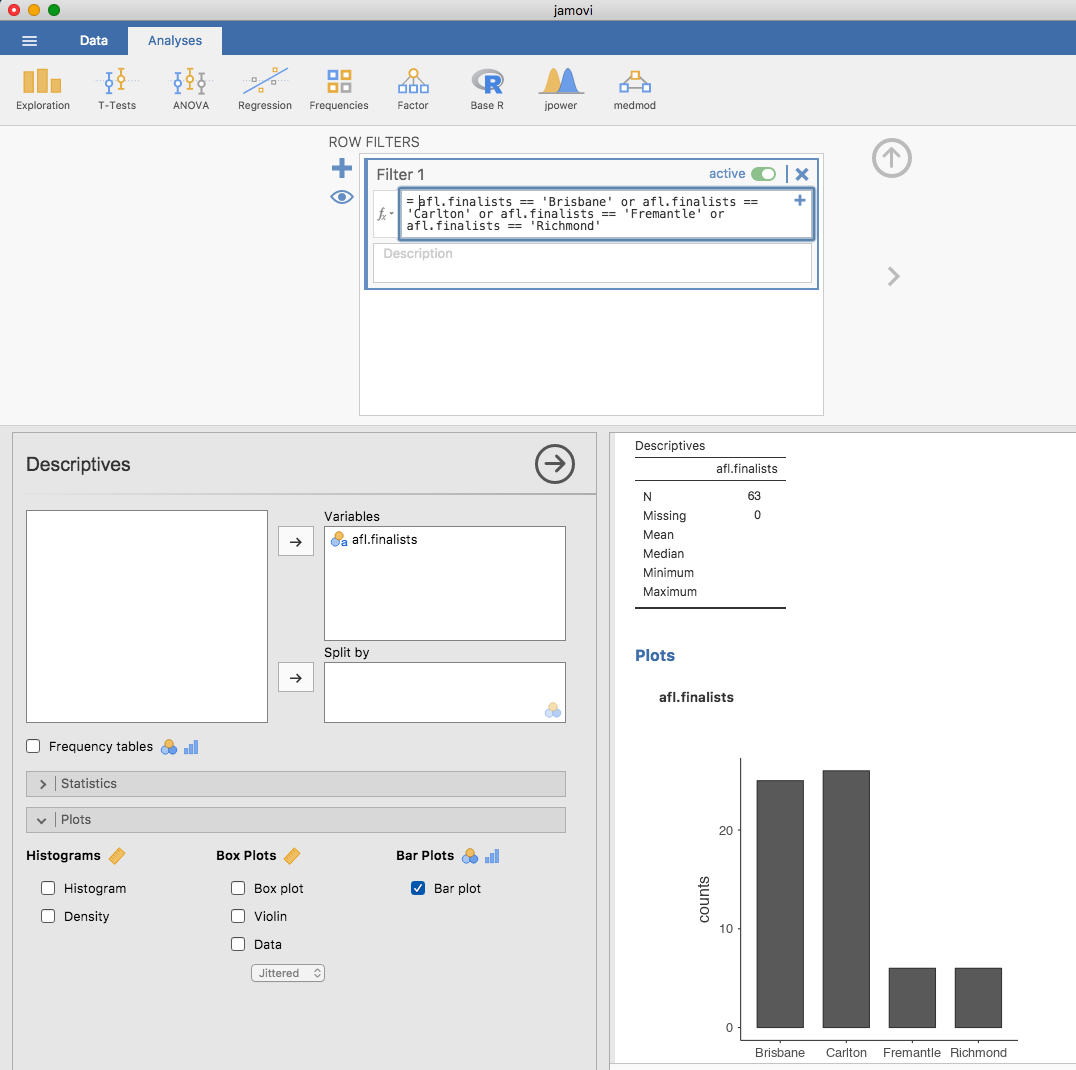
\epsfig{file = ../img/graphics/bar1.png, clip=true,width =13cm} 
\caption{Filtering to include just four AFL teams, and drawing a bar plot in jamovi}
\label{fig:bar1}
\HR
\end{center}
\end{figure}. 






%%%%%%%%%%%%%%%%%%%%%%%%%%%%%%%%%%%%%%%%%%%%%%%%%%%%%%%%%%%%%%%%%%%%%%%%%%%%%%%%%%%%%%%%%%
\iffalse % don't compile next parts - until ready! Move this code down as you revise....
%%%%%%%%%  when finished remove  /fi from the bottom of the tex filehttps://v2.overleaf.com/project/5b1c284b61f63b18810821bb
%%%%%%%%%%%%%%%%%%%%%%%%%%%%%%%%%%%%%%%%%%%%%%%%%%%%%%%%%%%%%%%%%%%%%%%%%%%%%%%%%%%%%%%%%%

\section{Scatterplots\label{sec:scatterplots}}

\keyterm{Scatterplots} are a simple but effective tool for visualising data. We've already seen scatterplots in this chapter, when using the \rtext{plot()} function to draw the \rtext{Fibonacci} variable as a collection of dots (Section~\ref{sec:introplotting}). However, for the purposes of this section I have a slightly different notion in mind. Instead of just plotting one variable, what I want to do with my scatterplot is display the relationship between {\it two} variables, like we saw with the figures in the section on correlation (Section~\ref{sec:correl}). It's this latter application that we usually have in mind when we use the term ``scatterplot''. In this kind of plot, each observation corresponds to one dot: the horizontal location of the dot plots the value of the observation on one variable, and the vertical location displays its value on the other variable. In many situations you don't really have a clear opinions about what the {\it causal} relationship is (e.g., does A cause B, or does B cause A, or does some other variable C control both A and B). If that's the case, it doesn't really matter which variable you plot on the x-axis and which one you plot on the y-axis. However, in many situations you do have a pretty strong idea which variable you think is most likely to be causal, or at least you have some suspicions in that direction. If so, then it's conventional to plot the cause variable on the x-axis, and the effect variable on the y-axis. With that in mind, let's look at how to draw scatterplots in \R, using the same \rtext{parenthood} data set (i.e. \filename{parenthood.Rdata}) that I used when introducing the idea of correlations.

\begin{figure}[t]
\begin{center}
\begin{tabular}{cc}
\epsfig{file = ../img/graphics2/scatter1b.eps, clip=true,width = 7cm} &
\epsfig{file = ../img/graphics2/scatter2b.eps, clip=true,width = 7cm} \\ (a) & (b) \\
\end{tabular}
\caption{Two different scatterplots: (a) the default scatterplot that \R\ produces, (b) one that makes use of several options for fancier display.}
\HR
\label{fig:scatter}
\end{center}
\end{figure}

Suppose my goal is to draw a scatterplot displaying the relationship between the amount of sleep that I get (\rtext{dan.sleep}) and how grumpy I am the next day (\rtext{dan.grump}). As you might expect given our earlier use of \rtext{plot()} to display the \rtext{Fibonacci} data, the function that we use is the \rtext{plot()} function, but because it's a generic function all the hard work is still being done by the \rtext{plot.default()} function. In any case, there are two different ways in which we can get the plot that we're after. The first way is to specify the name of the variable to be plotted on the \rtext{x} axis and the variable to be plotted on the \rtext{y} axis. When we do it this way, the command looks like this:
\begin{rblock1} 
> @usr{plot( x = parenthood$dan.sleep,}   # data on the x-axis
+ @usr{      y = parenthood$dan.grump}    # data on the y-axis
+ @usr{)}  
\end{rblock1}
The second way do to it is to use a ``formula and data frame'' format, but I'm going to avoid using it.\FOOTNOTE{The reason is that there's an annoying design flaw in the way the \rtextsmall{plot()} function handles this situation. The problem is that the \rtextsmall{plot.formula()} function uses different names to for the arguments than the \rtextsmall{plot()} function expects. As a consequence, you can't specify the formula argument by name. If you just specify a formula as the first argument without using the name it works fine, because the \rtextsmall{plot()} function thinks the formula corresponds to the \rtextsmall{x} argument, and the \rtextsmall{plot.formula()} function thinks it corresponds to the \rtextsmall{formula} argument; and surprisingly, everything works nicely. But the moment that you, the user, tries to be unambiguous about the name, one of those two functions is going to cry.} For now, let's just stick with the \rtext{x} and \rtext{y} version. If we do this, the result is the very basic scatterplot shown in Figure~\ref{fig:scatter}a. This serves fairly well, but there's a few customisations that we probably want to make in order to have this work properly. As usual, we want to add some labels, but there's a few other things we might want to do as well. Firstly, it's sometimes useful to rescale the plots. In Figure~\ref{fig:scatter}a \R\ has selected the scales so that the data fall neatly in the middle. But, in this case, we happen to know that the grumpiness measure falls on a scale from 0 to 100, and the hours slept falls on a natural scale between 0 hours and about 12 or so hours (the longest I can sleep in real life). So the command I might use to draw this is:
\begin{rblock1}
> @usr{plot( x = parenthood$dan.sleep,}         # data on the x-axis
+ @usr{      y = parenthood$dan.grump,}         # data on the y-axis
+ @usr{      xlab = "My sleep (hours)",}        # x-axis label
+ @usr{      ylab = "My grumpiness (0-100)",}   # y-axis label
+ @usr{      xlim = c(0,12),}                   # scale the x-axis
+ @usr{      ylim = c(0,100),}                  # scale the y-axis
+ @usr{      pch = 20,}                         # change the plot type
+ @usr{      col = "gray50",}                   # dim the dots slightly
+ @usr{      frame.plot = FALSE}                # don't draw a box
+ @usr{)}
\end{rblock1}
This command produces the scatterplot in Figure~\ref{fig:scatter}b, or at least very nearly. What it doesn't do is draw the line through the middle of the points. Sometimes it can be very useful to do this, and I can do so using \rtext{lines()}, which is a low level plotting function. Better yet, the arguments that I need to specify are pretty much the exact same ones that I use when calling the \rtext{plot()} function. That is, suppose that I want to draw a line that goes from the point (4,93) to the point (9.5,37). Then the \rtext{x} locations can be specified by the vector \rtext{c(4,9.5)} and the \rtext{y} locations correspond to the vector \rtext{c(93,37)}. In other words, I use this command:
\begin{rblock1}
> @usr{lines( x = c(4,9.5),}   # the horizontal locations
+ @usr{       y = c(93,37),}   # the vertical locations
+ @usr{       lwd = 2}         # line width
+ @usr{)}
\end{rblock1}
And when I do so, \R\ plots the line over the top of the plot that I drew using the previous command. In most realistic data analysis situations you absolutely don't want to just guess where the line through the points goes, since there's about a billion different ways in which you can get \R\ to do a better job. However, it does at least illustrate the basic idea. 


\begin{figure}[t]
\begin{center}
\epsfig{file = ../img/graphics2/fancyscatter.eps, clip=true,width = 10cm}
\caption{A fancy scatterplot drawn using the \rtext{scatterplot()} function in the \rtext{car} package.}
\HR
\label{fig:fancyscatter}
\end{center}
\end{figure}

One possibility, if you do want to get \R\ to draw nice clean lines through the data for you, is to use the \rtext{scatterplot()} function in the \rtext{car} package. Before we can use \rtext{scatterplot()} we need to load the package:
\begin{rblock1}
> @usr{library( car )}
\end{rblock1}
Having done so, we can now use the function. The command we need is this one:
\begin{rblock1}
> @usr{scatterplot( dan.grump ~ dan.sleep,}
+ @usr{             data = parenthood, }
+ @usr{             smooth = FALSE}
+ @usr{)}
\end{rblock1}
The first two arguments should be familiar: the first input is a formula (\rtextverb#dan.grump ~ dan.sleep#) telling \R\ what variables to plot,\FOOTNOTE{You might be wondering why I haven't specified the argument name for the formula. The reason is that there's a bug in how the \rtextsmall{scatterplot()} function is written: under the hood there's one function that expects the argument to be named \rtextsmall{x} and another one that expects it to be called \rtextsmall{formula}. I don't know why the function was written this way, but it's not an isolated problem: this particular kind of bug repeats itself in a couple of other functions (you'll see it again in Chapter~\ref{ch:ttest}). The solution in such cases is to omit the argument name: that way, one function ``thinks'' that you've specified \rtextsmall{x} and the other one ``thinks'' you've specified \rtextsmall{formula} and everything works the way it's supposed to. It's not a great state of affairs, I'll admit, but it sort of works.} and the second specifies a \rtext{data} frame. The third argument \rtext{smooth} I've set to \rtext{FALSE} to stop the \rtext{scatterplot()} function from drawing a fancy ``smoothed'' trendline (since it's a bit confusing to beginners). The scatterplot itself is shown in Figure~\ref{fig:fancyscatter}. As you can see, it's not only drawn the scatterplot, but its also drawn boxplots for each of the two variables, as well as a simple line of best fit showing the relationship between the two variables. 







 

\SUBSECTION{More elaborate options}


Often you find yourself wanting to look at the relationships between several variables at once. One useful tool for doing so is to produce a \keyterm{scatterplot matrix}, analogous to the correlation matrix. 
\begin{rblock1}
> @usr{cor( x = parenthood )} # calculate correlation matrix
             dan.sleep  baby.sleep   dan.grump         day
dan.sleep   1.00000000  0.62794934 -0.90338404 -0.09840768
baby.sleep  0.62794934  1.00000000 -0.56596373 -0.01043394
dan.grump  -0.90338404 -0.56596373  1.00000000  0.07647926
day        -0.09840768 -0.01043394  0.07647926  1.00000000
\end{rblock1}
We can get a the corresponding scatterplot matrix by using the \rtext{pairs()} function:\FOOTNOTE{Yet again, we could have produced this output using the \rtextsmall{plot()} function: when the \rtextsmall{x} argument is a data frame containing numeric variables only, then the output is a scatterplot matrix. So, once again, what I could have done is just type \rtextsmall{plot( parenthood )}.}
\begin{rblock1}
> @usr{pairs( x = parenthood )} # draw corresponding scatterplot matrix  
\end{rblock1}
The output of the \rtext{pairs()} command is shown in Figure~\ref{fig:pairs}.  An alternative way of calling the \rtext{pairs()} function, which can be useful in some situations, is to specify the variables to include using a one-sided formula. For instance, this
\begin{rblock1}
> @usr{pairs( formula = ~ dan.sleep + baby.sleep + dan.grump,}
+ @usr{       data = parenthood}
+ @usr{)}
\end{rblock1}
would produce a $3 \times 3$ scatterplot matrix that only compare \rtext{dan.sleep}, \rtext{dan.grump} and \rtext{baby.sleep}. Obviously, the first version is much easier, but there are cases where you really only want to look at a few of the variables, so it's nice to use the formula interface.


\begin{figure}
\begin{center}
\epsfig{file = ../img/graphics2/pairs3.eps,clip=true, width = 14cm}
\caption{A matrix of scatterplots produced using \rtext{pairs()}.}
\HR
\label{fig:pairs}
\end{center}
\end{figure}




\SUBSECTION{Changing global settings using \rtext{par()}\label{sec:par}}

Altering the margins to the plot is actually a somewhat more complicated exercise than you might think. In principle it's a very simple thing to do: the size of the margins is governed by a graphical parameter called \rtext{mar}, so all we need to do is alter this parameter. First, let's look at what the \rtext{mar} argument specifies. The \rtext{mar} argument is a vector containing four numbers: specifying the amount of space at the bottom, the left, the top and then the right. The units are ``number of `lines'". The default value for \rtext{mar} is \rtext{c(5.1, 4.1, 4.1, 2.1)}, meaning that \R\ leaves 5.1 ``lines'' empty at the bottom, 4.1 lines on the left and the bottom, and only 2.1 lines on the right. In order to make more room at the bottom, what I need to do is change the first of these numbers. A value of 10.1 should do the trick. 

So far this doesn't seem any different to the other graphical parameters that we've talked about. However, because of the way that the traditional graphics system in \R\ works, you need to specify what the margins will be {\it before} calling your high-level plotting function. Unlike the other cases we've see, you can't treat \rtext{mar} as if it were just another argument in your plotting function. Instead, you have to use the \rtext{par()} function to change the graphical parameters beforehand, and only then try to draw your figure. In other words, the first thing I would do is this:
\begin{rblock1} 
> @usr{par( mar = c( 10.1, 4.1, 4.1, 2.1) )}
\end{rblock1}
There's no visible output here, but behind the scenes \R\ has changed the graphical parameters associated with the current device (remember, in \R\ terminology all graphics are drawn onto a ``device''). Now that this is done, we could use the exact same command as before, but this time you'd see that the labels all fit, because \R\ now leaves twice as much room for the labels at the bottom. However, since I've now figured out how to get the labels to display properly, I might as well play around with some of the other options, all of which are things you've seen before:
\begin{rblock1}
> @usr{barplot( height = freq,}                      # the data to plot 
+ @usr{         names.arg = teams,}                  # label the plots
+ @usr{         las = 2, }                           # rotate the labels
+ @usr{         ylab = "Number of Finals", }         # y axis label
+ @usr{         main = "Finals Played, 1987-2010",}  # figure title
+ @usr{         density = 10, }                      # shade the bars
+ @usr{         angle = 20}                          # shading lines angle
+ @usr{)}
\end{rblock1}
However, one thing to remember about the \rtext{par()} function is that it doesn't just change the graphical parameters for the current {\it plot}. Rather, the changes pertain to any subsequent plot that you draw onto the same {\it device}. This might be exactly what you want, in which case there's no problem. But if not, you need to reset the graphical parameters to their original settings. To do this, you can either close the device (e.g., close the window, or click the ``Clear All'' button in the Plots panel in Rstudio) or you can reset the graphical parameters to their original values, using a command like this:
\begin{rblock1}
> @usr{par( mar = c(5.1, 4.1, 4.1, 2.1) )}
\end{rblock1}


\section{Saving image files using \R\ and Rstudio~\label{sec:saveimage}}

Hold on, you might be thinking. What's the good of being able to draw pretty pictures in \R\ if I can't save them and send them to friends to brag about how awesome my data is? How do I save the picture? This is another one of those situations where the easiest thing to do is to use the Rstudio tools.

If you're running \R\ through Rstudio, then the easiest way to save your image is to click on the ``Export'' button in the Plot panel (i.e., the area in Rstudio where all the plots have been appearing). When you do that you'll see a menu that contains the options ``Save Plot as PDF'' and ``Save Plot as Image''. Either version works. Both will bring up dialog boxes that give you a few options that you can play with, but besides that it's pretty simple. 

This works pretty nicely for most situations. So, unless you're filled with a burning desire to learn the low level details, feel free to skip the rest of this section.

\SUBSECTION{The ugly details \advanced} 

As I say, the menu-based options should be good enough for most people most of the time. However, one day you might want to be a bit more sophisticated, and make use of \R's image writing capabilities at a lower level. In this section I'll give you a very basic introduction to this. In all honesty, this barely scratches the surface, but it will help a little bit in getting you started if you want to learn the details. 

Okay, as I hinted earlier, whenever you're drawing pictures in \R\ you're deemed to be drawing {\it to} a device of some kind.  There are devices that correspond to a figure drawn on screen, and there are devices that correspond to graphics files that \R\ will produce for you. For the purposes of this section I'll assume that you're using the default application in either Windows or Mac OS, not Rstudio. The reason for this is that my experience with the graphical device provided by Rstudio has led me to suspect that it still has a bunch on non-standard (or possibly just undocumented) features, and so I don't quite trust that it always does what I expect. I've no doubt they'll smooth it out later, but I can honestly say that I don't quite get what's going on with the \rtext{RStudioGD} device.  In any case, we can ask \R\ to list all of the graphics devices that currently exist, simply by using the command \rtext{dev.list()}. If there are no figure windows open, then you'll see this:
\begin{rblock1}
> @usr{dev.list()}
NULL
\end{rblock1}
which just means that \R\ doesn't have any graphics devices open. However, suppose if you've just drawn a histogram and you type the same command, \R\ will now give you a different answer. For instance, if you're using Windows:
\begin{rblock1}
> @usr{hist( afl.margins )}
> @usr{dev.list()}
windows 
      2
\end{rblock1}
What this means is that there is one graphics device (device 2) that is currently open, and it's a figure window. If you did the same thing on a Mac, you get basically the same answer, except that the name of the device would be \rtextoutput{quartz} rather than \rtextoutput{windows}. If you had several graphics windows open (which, incidentally, you can do by using the \rtext{dev.new()} command) then you'd see something like this:
\begin{rblock1}
> @usr{dev.list()}
windows windows windows  
      2       3       4 
\end{rblock1}
Okay, so that's the basic idea behind graphics devices. The key idea here is that graphics files (like JPEG images etc) are {\it also} graphics devices as far as \R\ is concerned. So what you want to do is to {\it copy} the contents of one graphics device to another one. There's a command called \rtext{dev.copy()} that does this, but what I'll explain to you is a simpler one called \rtext{dev.print()}. It's pretty simple:

\begin{rblock1}
> @usr{dev.print( device = jpeg, }             # what are we printing to?
+ @usr{           filename = "thisfile.jpg",}  # name of the image file
+ @usr{           width = 480, }               # how many pixels wide should it be
+ @usr{           height = 300}                # how many pixels high should it be
+ @usr{)}
\end{rblock1}
This takes the ``active'' figure window, copies it to a jpeg file (which \R\ treats as a device) and then closes that device. The \rtext{filename = "thisfile.jpg"} part tells \R\ what to name the graphics file, and the \rtext{width = 480} and \rtext{height = 300} arguments tell \R\ to draw an image that is 300 pixels high and 480 pixels wide. If you want a different kind of file, just change the device argument from \rtext{jpeg} to something else. \R\ has devices for \rtext{png}, \rtext{tiff} and \rtext{bmp} that all work in exactly the same way as the \rtext{jpeg} command, but produce different kinds of files. Actually, for simple cartoonish graphics like this histogram, you'd be better advised to use PNG or TIFF over JPEG. The JPEG format is very good for natural images, but is wasteful for simple line drawings. The information above probably covers most things you might want to. However, if you want more information about what kinds of options you can specify using \R, have a look at the help documentation by typing \rtext{?jpeg} or \rtext{?tiff} or whatever.


\section{Summary}

Perhaps I'm a simple minded person, but I love pictures. Every time I write a new scientific paper, one of the first things I do is sit down and think about what the pictures will be. In my head, an article is really just a sequence of pictures, linked together by a story. All the rest of it is just window dressing. What I'm really trying to say here is that the human visual system is a very powerful data analysis tool. Give it the right kind of information and it will supply a human reader with a massive amount of knowledge very quickly. Not for nothing do we have the saying ``a picture is worth a thousand words''. With that in mind, I think that this is one of the most important chapters in the book. The topics covered were:

\begin{itemize}
\item {\it Basic overview to \R\ graphics}. In Section~\ref{sec:rgraphics} we talked about how graphics in \R\ are organised, and then moved on to the basics of how they're drawn in Section~\ref{sec:introplotting}.
\item {\it Common plots}. Much of the chapter was focused on standard graphs that statisticians like to produce: histograms (Section~\ref{sec:hist}), stem and leaf plots (Section~\ref{sec:stem}), boxplots (Section~\ref{sec:boxplots}), scatterplots (Section~\ref{sec:scatterplots}) and bar graphs (Section~\ref{sec:bargraph}).
\item {\it Saving image files}. The last part of the chapter talked about how to export your pictures (Section~\ref{sec:saveimage})
\end{itemize} 

\noindent
One final thing to point out. At the start of the chapter I mentioned that \R\ has several completely distinct systems for drawing figures. In this chapter I've focused on the {\it traditional} graphics system. It's the easiest one to get started with: you can draw a histogram with a command as simple as \rtext{hist(x)}. However, it's not the most powerful tool for the job, and after a while most \R\ users start looking to shift to fancier systems. One of the most popular graphics systems is provided by the \rtext{ggplot2} package (see \url{http://ggplot2.org/}), which is loosely based on ``The grammar of graphics'' \cite{Wilkinson2006}. It's not for novices: you need to have a pretty good grasp of \R\ before you can start using it, and even then it takes a while to really get the hang of it. But when you're finally at that stage, it's worth taking the time to teach yourself, because it's a much cleaner system.




/fi %remove when finished revising chapter

